\documentclass[../main/main.tex]{subfiles}

\raggedbottom

\makeatletter
\renewcommand{\@chapapp}{\'Electrocin\'etique -- chapitre}
\makeatother

\begin{document}
\setcounter{chapter}{0}

\chapter{Circuits \'electriques dans l'ARQS}

Pendant toute cette année nous nous plaçons dans un cadre particulier pour
l'étude de l'électrocinétique, celui de l'\textit{approximation des régimes
quasi-stationnaires}, ou ARQS. Dans ce premier chapitre, nous nous attachons à
définir ce cadre et donnons les lois générales des circuits électriques que nous
pouvons alors établir.

\section{Courant électrique et intensité}
\subsection{Charge électrique}

\begin{tcbraster}[raster columns=2, raster equal height=rows]
    \begin{defi}[label=def:q, sidebyside]{charge électrique}
        La charge électrique d'une particule, notée $q$, est une grandeur
        scalaire, caractérisant sa sensibilité aux interactions
        électromagnétiques.
        \tcblower
        \tcbsubtitle[before skip=\baselineskip,
        colback=green!50!black,
        colframe=green!50!black]{Unités}
        La charge électrique s'exprime en Coulomb, de symbole C.
    \end{defi}
    \begin{exem}[label=exem:q]{matière ordinaire}
        La matière ordinaire est constituée d'atomes, formés par~:
        \begin{itemize}
            \item des \textbf{neutrons}, électriquement neutres (de charge nulle)~;
            \item des \textbf{protons}, de charge positive et fondamentale~: $e =
                \SI{1.6e-19}{C}$~;
            \item des \textbf{électrons}, de charge négative opposée à celle des
                protons
        \end{itemize}
    \end{exem}
\end{tcbraster}
\begin{prop}[label=prop:q]{charge électrique et conservation}
    Un système électrique de charge totale $Q$ possède les propriétés
    suivantes~:
    \begin{enumerate}
        \item $Q$ est \textbf{algébrique}~: elle peut être $\lessgtr 0$~;
        \item $Q$ est \textbf{additive}~: $N$ particules de charges $q_{1, …,
            N}$ forment une charge $Q = \sum_{i=1}^{N} q_i$~;
        \item $Q$ est quantifiée~: $Q = k\times e$ avec $k \in \Zb$ et $e =
            \SI{1.6e-19}{C}$~;
        \item \fbox{Si le système est isolé, alors $Q$ est constante.}
    \end{enumerate}
\end{prop}

\subsection{Courant électrique}
\begin{tcbraster}[raster columns=2, raster equal height=rows]
    \begin{defi}[label=def:courant]{courant électrique}
        Le courant électrique est un \textbf{mouvement d'ensemble} de particules
        chargées, appelées \textit{porteurs de charges}, dû à une action
        extérieure, le champ électrique $\Ef$ (voir 2ème année).
    \end{defi}
    \begin{exem}[label=exem:porteurs]{porteurs de charges}
        On étudiera deux types de porteurs~:
        \begin{enumerate}
            \item Les \textbf{électrons libres} dans les conducteurs métalliques~;
            \item Les \textbf{ions en solutions} dites électrolytiques.
        \end{enumerate}
    \end{exem}
\end{tcbraster}

\subsection{Sens conventionnel du courant}

\begin{tcbraster}[raster columns=3, raster equal height=rows]
    \begin{tcolorbox}[blankest, raster multicolumn=2, valign=center]
    Les particules sont déplacées par un champ électrique $\Ef$ selon le sens
    algébrique de leur charge, avec une force $\Ff = q\Ef$ (voir mécanique
    première année)~: les charges avec $q>0$ sont déplacées dans le même sens
    que $\Ef$, celles de $q<0$ dans le sens opposé. Ils apportent cependant la
    \textit{même variation de charge} en valeur absolue. Avant de connaître
    quelles particules se déplaçaient dans les circuits électriques (les
    électrons), il a fallu choisir un sens conventionnel~:
    \end{tcolorbox}    
    \begin{defi}[label=def:sensconv]{sens conventionnel}
        Le sens conventionnel du courant est le sens de déplacement des porteurs
        charges positives (réels ou hypothétiques). Les charges négatives se
        déplacent en sens contraire.
    \end{defi}
\end{tcbraster}

\subsection{Intensité du courant}
\begin{tcbraster}[raster columns=3, raster equal height=rows]
    
\begin{defi}[label=def:intensité, sidebyside, raster multicolumn=2]{intensité
    d'un courant}

    L'intensité électrique quantifie le \textbf{débit} de charges à travers une
    \underline{section orientée}, c'est-à-dire un \textbf{nombre de charges par
    unité de temps} dans la section étudiée. Une charge est comptée $+q$
    si elle traverse la section dans le même sens que son orientation (avec $q
    \lessgtr 0$), et $-q$ sinon.

    \tcblower
    \tcbsubtitle[before skip=\baselineskip,
    colback=green!50!black,
    colframe=green!50!black]{Unités}
    L'intensité se mesure en Ampère, de symbole A. De la définition, on a
    \SI{1}{A} = \SI{1}{C.s^{-1}}.
    \tcbsubtitle[before skip=\baselineskip,
    colback=green!50!black,
    colframe=green!50!black]{Notation}
    Par convention, $i$ si elle varie, $I$ si elle est fixe.
\end{defi}
\begin{prop}[label=prop:intensité]{expression de l'intensité}

    Soit un système électrique de \textbf{section orientée} $S$ traversée par
    des charges électriques. Si une quantité de charge $\delta q$ la traverse
    entre deux instants $t$ et $t + \delta t$, l'intensité $i$ du courant sera
    $i = \delta q/\delta t$, d'où en prenant la limite
    \[ \boxed{i(t) = \underset{\de t\rightarrow0}{\lim} \frac{\delta q}{\delta t} =
    \dv{q}{t}}\]
\end{prop}
\end{tcbraster}
\begin{tcbraster}[raster columns=2, raster equal height=rows]
    \begin{impl}[label=impl:intensconv]{signe et sens réel}
        Si $i > 0$, $\de q > 0$~: entre $t$ et $t+\d t$ il y a eu une traversée de
        charges avec résultante positive \textit{dans le sens orienté}. Comme le
        sens conventionnel est \textbf{celui des charges positives}, on retiendra
        \begin{itemize}
            \item si $i > 0$, le sens conventionnel est respecté~;
            \item si $i < 0$, le sens conventionnel est opposé à l'orientation
                choisie.
        \end{itemize}
    \end{impl}
    \begin{nota}[label=nota:intensconv]{représentation du sens}
        En représentant un fil électrique par un trait rectiligne, on oriente la
        section avec une flèche. La grandeur ainsi définie peut être $\lessgtr 0$.
        Si on la flèche dans l'autre sens, sa valeur est opposée.
        \tcblower
        \begin{center}
            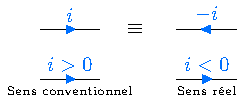
\includegraphics[width=\linewidth]{intensconv}
        \end{center}
    \end{nota}
\end{tcbraster}
\begin{impo}[label=impo:courantintensité]{courant et intensité}
    Il vous faut savoir différencier le courant et l'intensité du courant~:
    \begin{imposide}
        Le courant est le \textit{phénomène physique}.
        \tcblower
        L'intensité en est la \textit{quantification algébrique}.
    \end{imposide}
\end{impo}
\begin{tcbraster}[raster columns=2, raster equal height=rows]
    \begin{odgr}[label=odgr:intensité]{intensités}
        Les valeurs mesurées sont~:

        \begin{itemize}
            \item $\approx \SI{1}{mA}$ pour l'électronique du quotidien
                (téléphone)~;
            \item $\SIrange{1}{10}{A}$ pour l'électroménager (four,
                aspirateur…)~;
            \item $\approx \SI{e2}{A}$ pour l'électrotechnique (TGV~:
                \SIrange{500}{1000}{A}).
        \end{itemize}

        Le seuil létal pour le corps dépend de la durée de traversée, mais est
        \textbf{très faible}~: \SI{40}{mA} pendant 3 secondes, ou \SI{300}{mA}
        pendant \SI{0.1}{seconde}.

    \end{odgr}
    \begin{NCcexe}[width=\linewidth]{Exercice d'application}

        Un générateur délivre une intensité $I = \SI{3.0}{A}$. Quel est le
        nombre d'électrons émis chaque seconde~? Quelle durée faut-il à ce
        générateur pour émettre \num{1000} électrons~?

        \tcblower
        \vspace*{3cm}
    \end{NCcexe}
\end{tcbraster}

\section{Tension et potentiel}
\subsection{Définition}
\begin{tcbraster}[raster columns=5, raster equal height=rows]
    \begin{defi}[label=def:tension, sidebyside, raster multicolumn=3]{potentiel et tension}

        On appelle \textbf{potentiel} électrique la grandeur physique reliant la
        capacité d'un point à attirer les charges négatives~: plus le potentiel
        est élevé plus il les attire. On appelle \textbf{tension} ou
        \textbf{différence de potentiel} entre deux points la différence entre
        les valeurs du potentiel en chacun des points.

        \tcblower
        \tcbsubtitle[before skip=\baselineskip,
        colback=green!50!black,
        colframe=green!50!black]{Unités}
        Le potentiel, et par extension la différence de potentiel, s'exprime en
        Volt, de symbole V.
        \tcbsubtitle[before skip=\baselineskip,
        colback=green!50!black,
        colframe=green!50!black]{Notation}
        $u$ si variable, $U$ sinon.
        \tcbsubtitle[before skip=\baselineskip,
        colback=green!50!black,
        colframe=green!50!black]{En pratique}
        \textbf{Seules les tensions se mesurent}
    \end{defi}
    \begin{nota}[label=nota:tension, raster multicolumn=2]{potentiel et tension}

        Il est convenu d'écrire le potentiel en un point A~: $V_A$, et la
        tension \textbf{entre les points} A et B~: $U_{AB} = V_A - V_B$. Sur un
        schéma, la tension est représentée par une flèche partant du
        \textbf{second potentiel vers le premier}.

        \tcblower
        \begin{center}
            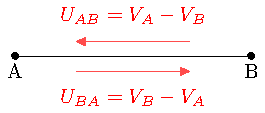
\includegraphics[width=\linewidth]{tensionconv}
        \end{center}
    \end{nota}
\end{tcbraster}
\begin{tcbraster}[raster columns=2, raster equal height=rows]
    \begin{impl}[label=impl:tension]{signe d'une tension}

        \begin{itemize}
            \item $U_{AB} > 0$ si $V_A > V_B$ et inversement~;
            \item \fbox{$U_{AB} = - U_{BA}$}~;
            \item \fbox{$U_{AB} = U_{AC} + U_{CB}$}.
        \end{itemize}

        \textbf{Attention} cependant, la flèche est opposée au sens usuel pour
        un vecteur $\overrightarrow{AB}$.

    \end{impl}
    \begin{odgr}[label=odgr:tensions]{tensions}
        Les valeurs mesurées sont~:

        \begin{itemize}
            \item $\approx \SIrange{0.100}{5}{V}$ pour l'électronique du
                quotidien (téléphone)~;
            \item $\approx \SI{220}{V}$ pour l'électroménager (four,
                aspirateur…)~;
            \item $\approx \SIrange{100}{1000}{kV}$ pour l'électrotechnique
                (lignes hautes tensions).
        \end{itemize}

    \end{odgr}
\end{tcbraster}

\subsection{Référence du potentiel~: la masse}

\begin{tcbraster}[raster columns=2, raster equal height=rows]
    \begin{defi}[label=def:masse]{masse d'un circuit}

        L'origine des potentiels d'un circuit est appelée la \textbf{masse} du
        circuit. C'est le point où $V = 0$. Elle sert de référence et est
        choisie arbitrairement, les tensions pouvant être négatives, et permet
        la mesure des tensions.

    \end{defi}
    \begin{nota}[label=nota:masse]{représentation}

        Dans un circuit électrique, elle est représentée par l'un de ces deux
        symboles

        \begin{center}
            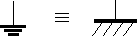
\includegraphics[width=\linewidth]{masse}
        \end{center}
    \end{nota}
\end{tcbraster}

\section{Analogie électro-hydraulique}

Les phénomènes régissant la tension et le courant électrique sont en tous points
semblables à ceux régissant le dénivelé et le courant dans un circuit
hydraulique. Cette vision permet de mieux comprendre le vocabulaire employé.

Considérons une analogie hydraulique~: dans une conduite d'eau horizontale entre
deux récipients, l'eau ne s'écoulera pas. Un courant d'eau apparaîtra si on
surélève l'un des récipients par rapport à l'autre, et ce courant sera
\textbf{vers le plus bas}. Le récipient surélevé va finir par se vider et le
courant d'eau cessera. C'est la \textbf{différence d'altitude} entre les deux
récipients qui permet la \textbf{circulation du courant}. Les deux sens ne sont
pas équivalents, le courant d'eau ne se produit spontanément que vers le bas.

Par analogie avec l'\textbf{altitude} $h$ de la canalisation, on définit le
\textbf{potentiel} électrique $V$. Ainsi, un courant électrique apparaît
spontanément dans le sens des \textbf{potentiels décroissants}. Pour que le
courant remonte les potentiels, il faut « pomper » les charges à l'aide d'un
générateur. L'équivalent électrique du dénivelé (différence d'altitudes) en
hydraulique est la tension (différence de potentiels). Voir ce site et
l'animation flash~: \href{https://www.pccl.fr/physique\_chimie\_college\_lycee/quatrieme/electricite/analogie\_hydraulique.htm}
{https://www.pccl.fr/physique\_chimie\_college\_lycee/quatrieme/electricite/}

\begin{figure}[h]
    \centering
    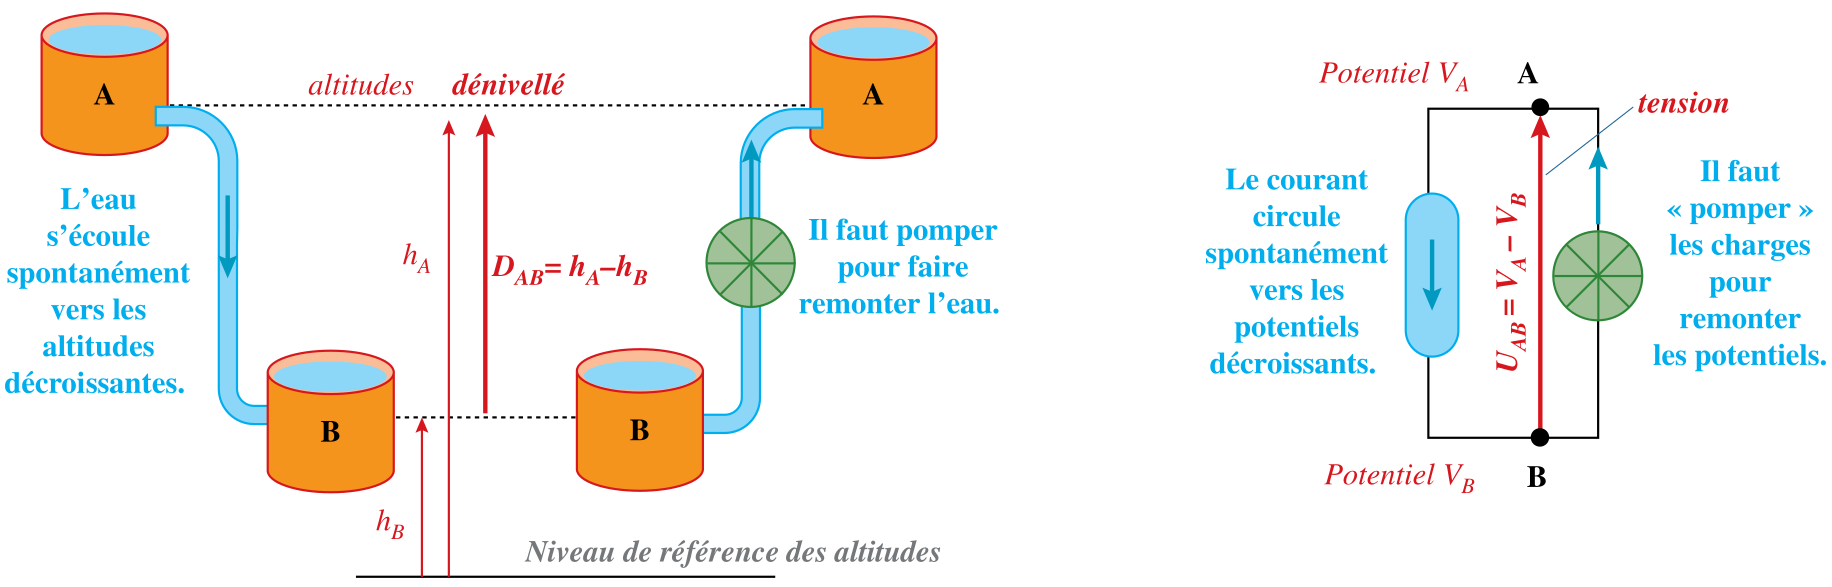
\includegraphics[width=\linewidth]{anal_elec-hydro.png}
    \label{fig:anal_elec-hydro}
\end{figure}

On définit de la même manière la puissance~: pour l'hydraulique, la puissance
d'un courant est égal au produit du dénivelé et du débit, en
électrocinétique on aura donc
\[\boxed{\left| P \right| = U\cdot I}\]
Nous discutons de son signe dans la section suivante.

\section{Vocabulaire des circuits électriques}
\subsection{La base}
\begin{tcbraster}[raster columns=2, raster equal height=rows]
    \begin{defi}[label=def:circuits]{base}

        \begin{itemize}[leftmargin=100pt]
            \item[\textbf{Circuit électrique}]: ensemble de composants
                électriques reliés entre eux par des fils métalliques
                conducteurs.
            \item[\textbf{Schéma électrique}]: représentation simplifiée d'un
                circuit dans laquelle les composants sont représentés par des
                symboles standardisés et les fils les reliant par des traits.
            \item[\textbf{Dipôle}]: composant électriques comportant deux bornes
                sur lesquelles sont branchés des fils conducteurs.
        \end{itemize}
    \end{defi}
    \begin{exem}[label=exem:circuits]{circuit et schéma}
        \begin{center}
            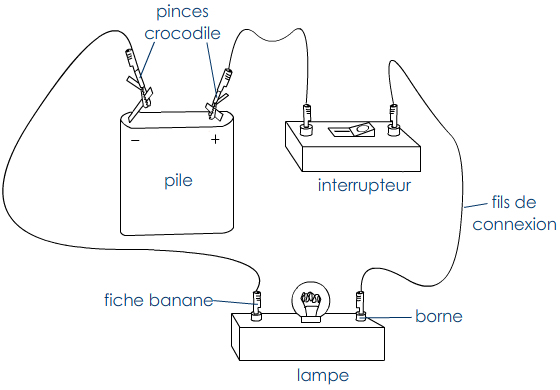
\includegraphics[width=.7\linewidth]{circuit_simple_dessin.jpg}
        \end{center}
        \tcblower
        \begin{center}
            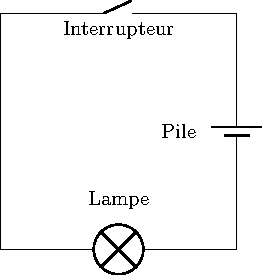
\includegraphics[width=.5\linewidth]{circuit_simple.pdf}
        \end{center}
    \end{exem}
\end{tcbraster}

\subsection{Décrire un circuit}
\begin{tcbraster}[raster columns=2, raster equal height=rows]
    
    \begin{defi}[label=def:descri]{description}
        \begin{itemize}[leftmargin=50pt]
            \item[\textbf{Nœud}]: point où se rejoignent au moins 3 fils.
            \item[\textbf{Branche}]: portion du circuit entre deux nœuds
                voisins.
            \item[\textbf{Maille}]: succession de branches partant et retournant
                au même point.
        \end{itemize}
    \end{defi}
    \begin{exem}[label=exem:descri]{description}
        \begin{center}
            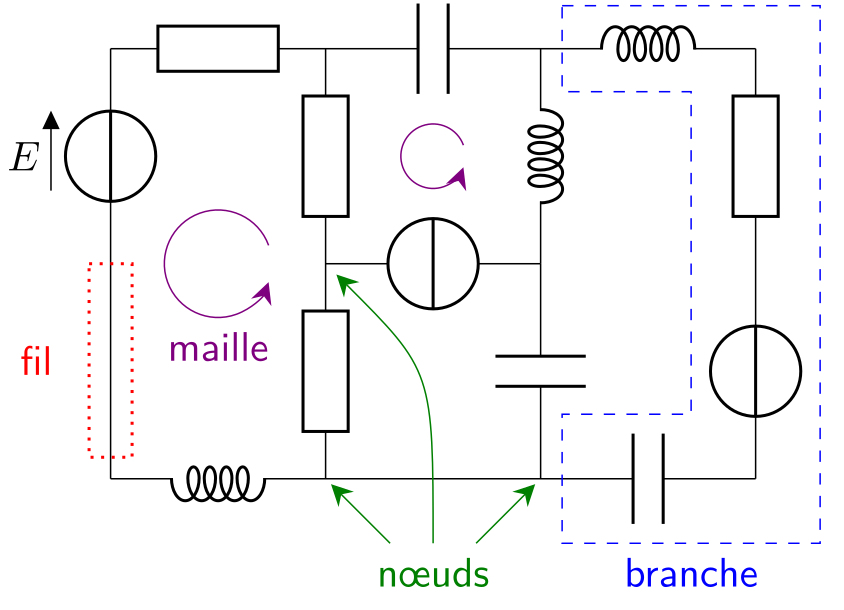
\includegraphics[width=\linewidth]{circuit_voca}
        \end{center}
    \end{exem}
\end{tcbraster}

\subsection{Conventions générateur et récepteur}
Chacune des orientations de l'intensité et de la tension est arbitraire. Pour
étudier le comportement d'un dipôle, il nous faut choisir une dernière
convention donnant l'orientation relative de la tension $u$ à ses bornes et de
l'intensité $i$ du courant la traversant. Celle-ci dépend de la nature
génératrice ou réceptrice d'un dipôle afin de respecter leurs physiques
respectives.

% ~; notamment, l'énergie étant conservée dans un circuit, on doit
% avoir un équilibre entre puissances fournies et reçues.

% \begin{defi}[label=def:convrg]{conventions selon dipôle}
%     Dans une maille d'un circuit, les puissances fournies et reçues
%     s'équilibrent, ce qui se traduit par $\DS \sum P_{\text{fournies}} =
%     \sum P_{\text{reçues}}$, avec les conventions~:
% 
%     \begin{tabularx}{\linewidth}{|Y*{2}{|Y}|}\hline
%         &
%         Dipôle \textcolor{ForestGreen}{récepteur} &
%         Dipôle \textcolor{CornflowerBlue}{générateur}
%         \\\hline
%         Convention récepteur
%         \smallbreak $\textcolor{orange}{P_{\text{reçue}}}$ &
%         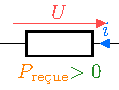
\includegraphics[width=3cm]{rconvr}
%          &
%         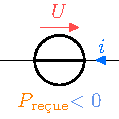
\includegraphics[width=3cm]{gconvr}
%         \\\hline
%         Convention générateur
%         \smallbreak $\textcolor{Purple}{P_{\text{fournie}}}$ &
%         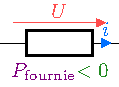
\includegraphics[width=3cm]{rconvg}
%          &
%         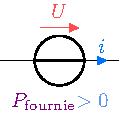
\includegraphics[width=3cm]{gconvg}
%         \\\hline
%     \end{tabularx}
% \end{defi}

\begin{defi}[label=def:convrg, sidebyside, righthand width=.3\linewidth]
    {conventions récepteur et générateur}
    En convention \textbf{récepteur}, l'intensité $i$ traversant un dipôle et la
    tension $u$ à ses bornes sont orientées en \textbf{sens contraires}.
    \bigbreak
    En convention \textbf{générateur}, l'intensité $i$ traversant un dipôle et la
    tension $u$ à ses bornes sont orientées en \textbf{dans le même sens}.
    \tcblower
    \begin{center}
        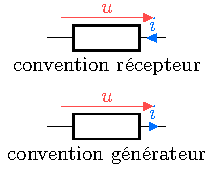
\includegraphics[width=\linewidth]{rgconv}
    \end{center}
\end{defi}

\subsection{Relation entre dipôles}
\begin{tcbraster}[raster columns=3, raster equal height=rows]
    
\begin{defi}[label=def:serdiv, valign lower=center, valign upper=center]
    {série et dérivation}

    Deux dipôles sont dits \textbf{en série} s'ils partagent \textbf{une et une
    seule borne} qui \textbf{n'est pas un nœud} (de laquelle ne part aucune
    autre branche).\vspace{10pt}

    \tcblower
    Deux dipôles sont dits \textbf{en dérivation/en parallèle} s'ils partagent
    leurs \textbf{deux bornes}.
\end{defi}
\begin{coro}[label=coro:serdiv, valign lower=center, valign upper=center]
    {série et dérivation}

    Deux dipôles \textbf{en série} sont traversés par la \textbf{même
    intensité}. \vspace{56pt}

    \tcblower

    Deux dipôles \textbf{en parallèle/dérivation} ont la \textbf{même tension} à
    leurs bornes.

\end{coro}
\begin{exem}[label=exem:serdiv]{série et dérivation}
    \begin{center}
        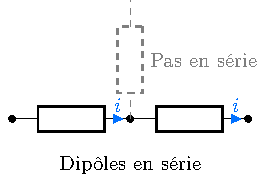
\includegraphics[width=\linewidth]{serie}
    \end{center}
    \tcblower
    \begin{center}
        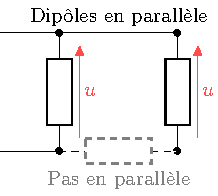
\includegraphics[width=\linewidth]{derivation}
    \end{center}
\end{exem}
\end{tcbraster}

    
\begin{rema}[label=rema:serdiv, halign=center]{série et dérivation}
    \textbf{Deux dipôles peuvent n'être ni en série, ni en dérivation.}
\end{rema}
\begin{NCcexe}[label=exer:serdiv]{Exercice d'application}

    \begin{minipage}{0.65\linewidth}
        
        Pour le schéma ci-dessous, indiquer si les couples de dipôles suivants
        sont en série, en parallèle ou ni l'un ni l'autre~: ($R_1$ et $R_0$) ;
        ($r_0$ et $r_2$) ; ($R_2$ et $R_0$) ; ($R_3$ et $r_2$) ; ($R_3$ et
        $R_2$).

    \end{minipage}
    \begin{minipage}{0.35\linewidth}
        \begin{center}
            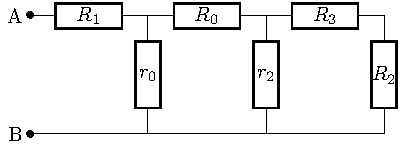
\includegraphics[width=\linewidth]{exer_serdiv}
        \end{center}
    \end{minipage}
    \tcblower
    \vspace*{2cm}
\end{NCcexe}

\subsection{Mesures de tensions et d'intensités}

\begin{prop}[label=prop:mesure, sidebyside]{voltmètre et ampèremètre}

   Une tension se mesure à l'aide d'un voltmètre, qui se branche entre les
   points A et B où on veut mesurer la tension, donc en parallèle du ou des
   dipôles qui s'y trouvent déjà. On dit souvent qu'«~\textbf{un voltmètre se
   monte en parallèle}~». Pour mesurer la tension $U_{AB}$ il faut placer la
   borne COM au point B. 

   \bigbreak

    Une intensité se mesure à l'aide d'un ampèremètre, qui se place directement
    dans la branche où on souhaite mesurer l'intensité~: on dit souvent
    qu'«~\textbf{un ampèremètre se monte en série}~». Le sens du courant affiché
    par l'ampèremètre est relié au sens de branchement.

    \tcblower
    \begin{center}
        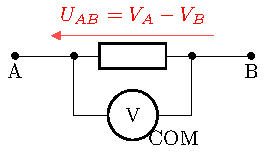
\includegraphics[width=\linewidth]{voltmetre}
    \end{center}
    \begin{center}
        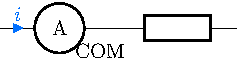
\includegraphics[width=\linewidth]{amperemetre}
    \end{center}
\end{prop}

\section{Lois fondamentales des circuits électriques dans l'ARQS}

\subsection{L'approximation des régimes quasi-stationnaires (ARQS)}

\begin{tcbraster}[raster columns=2, raster equal height=rows]
    \begin{loi}[label=loi:arqs]{ARQS}

        L'approximation des régimes quasi-stationnaires correspond à considérer
        que les variations des grandeurs électriques se propagent
        \textit{instantanément} dans la totalité d'un circuit. Si sa longueur
        totale est $L$ et si la fréquence de variation du signal électrique est
        $f$ (ou temps de variation $T$), l'ARQS est applicable si

        \[ L \ll \frac{c}{f} \Longleftrightarrow \boxed{L \ll cT} \Longleftrightarrow T \gg
        \frac{L}{c}\]
    \end{loi}
    \begin{demo}[label=demo:arqs]{ARQS}
    
        Dans un fil, les électrons sont mis en mouvement par un champ
        électrique. La théorie électromagnétique nous montre que le champ
        électrique est une onde qui se déplace à la célérité $c \approx
        \SI{3.00e8}{m.s^{-1}}$. Ainsi, la variation du potentiel dans un fil se
        fait à vitesse finie et il y a en général un \textbf{retard à la
        propagation}. Si le champ varie dans le temps avec une période $T$, il
        varie dans l'espace avec une période $\lambda = cT$. On peut alors
        considérer que le champ électrique est le même le long d'un fil si sa
        taille est beaucoup plus petite que la longueur d'onde $\lambda$.
    \end{demo}
\end{tcbraster}
\begin{NCcexe}[width=\linewidth]{Application}
    Vérifier si l'ARQS est valable pour les 3 cas suivants~:
    \begin{itemize}
        \item En travaux pratiques avec $f = \SI{1}{kHz}$~;
        \item Sur une ligne à haute tension de \SI{100}{km} à basse fréquence
            (\SI{50}{Hz})~;
        \item À l'intérieur d'une carte mère d'un ordinateur de \SI{10}{cm} à
            $f \approx \SI{1}{GHz}$.
    \end{itemize}
    \tcblower
    Oui, si $L \ll \SI{300}{km}$~; oui, si $L \ll \SI{6000}{km}$~; non, $Lf =
    \SI{1e8}{m.s^{-1}} \neg\ll c$.
\end{NCcexe}
\begin{defi}[label=def:regimecontvar, sidebyside]{régimes continu et variable}

    \textbf{Régime continu}~: toutes les intensités et les tensions du circuit
    sont constantes ou cours du temps.

    \tcblower

    \textbf{Régime variable}~: au moins une tension ou une intensité du circuit
    varie au cours du temps. Si on se place dans l'ARQS, on parle parfois de
    régime lentement variable.
\end{defi}

\subsection{Loi des nœuds}

Dans le cadre de l'ARQS, il ne peut y avoir d'accumulation de charges en un
point du circuit~: toutes les charges apportées par un courant doivent
immédiatement être évacuées par un autre courant, donnant lieu aux lois des
branches et des nœuds~:
\begin{loi}[label=loi:branche, sidebyside, halign upper=center]{loi des branches}
    \textbf{L'intensité est la même le long d'une branche}.
    \tcblower
    \begin{center}
        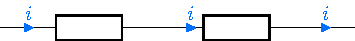
\includegraphics[width=\linewidth]{ldb}
    \end{center}
\end{loi}
\begin{loi}[label=loi:noeud, sidebyside, halign upper=center]{loi des nœuds}
    \textbf{La somme des intensités dirigées vers un nœud est égale à la somme de
    celles dirigées à l'opposé}, ou \textbf{la somme algébrique des intensités
    en un point est nulle}.
    \tcblower
    \begin{center}
        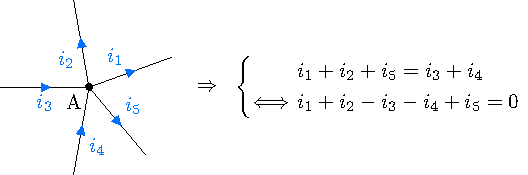
\includegraphics[width=\linewidth]{ldn}
    \end{center}
\end{loi}

\subsection{Loi des mailles}

Avec le principe d'additivité des tensions (implication \ref{impl:tension}), on
en déduit la loi des mailles.
\begin{loi}[label=loi:mailles, sidebyside, halign upper=center]{loi des mailles}

    \textbf{Dans une maille orientée, la somme algébrique des tensions est nulle
    }, ou \textbf{la somme des tensions dans le sens de la maille est égale à la
    somme des tensions dans le sens opposé}
    \tcblower
    \begin{center}
        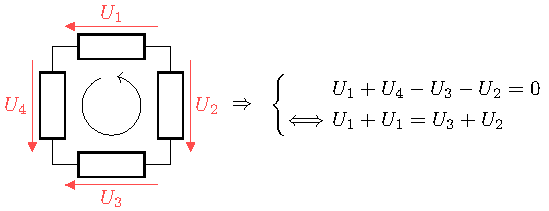
\includegraphics[width=\linewidth]{ldm}
    \end{center}
\end{loi}

\begin{NCcexe}[breakable]{Exercice d'application}

    \begin{minipage}{0.30\linewidth}
        Pour le circuit ci-contre, établir les liens entre les différents
        courants et les différentes tensions.
    \end{minipage}
    \begin{minipage}{0.70\linewidth}
        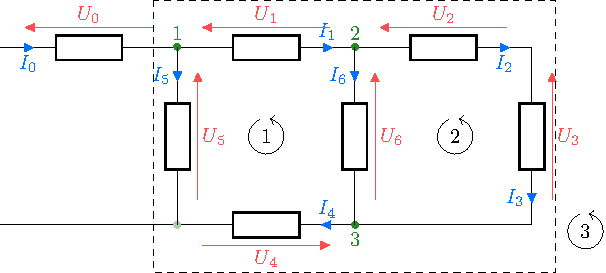
\includegraphics[width=\linewidth]{exer_ldnm}
    \end{minipage}
    \tcblower
    \begin{minipage}{0.47\linewidth}
        \begin{itemize}
            \item $I_2 = I_3$ par unicité à droite ;
            \item $I_0 = I_1 + I_5$ par LdN 1 ;
            \item $I_1 = I_2 + I_6$ par LdN 2 ;
            \item $I_3 + I_6 = I_4$ par LdN 3.
        \end{itemize}
        Le dernier nœud, non numéroté, donne une relation redondante avec les
        autres.
    \end{minipage}
    \hfill
    \begin{minipage}{0.47\linewidth}
        \begin{itemize}
            \item $U_4 + U_6 + U_1 = U_5$ par LdM 1 ;
            \item $U_3 + U_2 = U_6$ par LdM 2 ;
        \end{itemize}
        La LdM 3 donne une relation redondante avec les deux premières : $U_4
        + U_2 + U_3 + U_1 = U_5$ est la somme des deux.
    \end{minipage}
\end{NCcexe}

\subsection{Puissance électrocinétique}

\begin{defi}[label=def:puissance]{puissance récepteur, générateur}

    Un dipôle \textbf{fonctionne comme récepteur} s'il \textbf{reçoit de
    l'énergie} du reste système. Dans ce cas-là, sa puissance \textit{en
    convention récepteur} est $P_{\text{reçue}} = u\times i > 0$. Si après
    calcul une puissance reçue est négative, c'est que le dipôle est en fait
    générateur. \tcblower

    Un dipôle \textbf{fonctionne comme générateur} s'il \textbf{fournit de
    l'énergie} au reste système. Dans ce cas-là, sa puissance \textit{en
    convention générateur} est $P_{\rm fournie} = u\times i > 0$. Si après
    calcul une puissance fournie est négative, c'est que le dipôle est en fait
    récepteur.
    
\end{defi}

\begin{exem}[label=exem:convrg]{puissances}
    \begin{tabularx}{\linewidth}{|Y*{2}{|Y}|}\hline
        &
        Dipôle \textcolor{ForestGreen}{récepteur} &
        Dipôle \textcolor{CornflowerBlue}{générateur}
        \\\hline
        Convention récepteur
        \smallbreak $\textcolor{orange}{P_{\text{reçue}}}$ &
        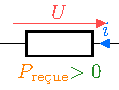
\includegraphics[width=3cm]{rconvr}
         &
        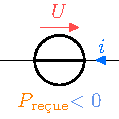
\includegraphics[width=3cm]{gconvr}
        \\\hline
        Convention générateur
        \smallbreak $\textcolor{Purple}{P_{\text{fournie}}}$ &
        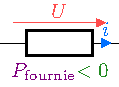
\includegraphics[width=3cm]{rconvg}
         &
        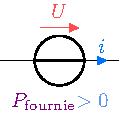
\includegraphics[width=3cm]{gconvg}
        \\\hline
    \end{tabularx}
\end{exem}

\begin{prop}[label=prop:puiss]{conservation de l'énergie}

    L'\textbf{énergie} est une \textbf{grandeur conservative}. Elle ne peut être
    crée ou détruite. Elle ne peut qu'être convertie d'une forme en une autre
    et/ou transférée d'un système à un autre. Il en découle que dans une maille,
    \textbf{les puissances reçues sont égales aux puissances émises},
    c'est-à-dire
    \[\boxed{\sum P_{\rm fournies} = \sum P_{\text{reçues}}}\]
\end{prop}

\end{document}
